\documentclass[a4paper,12pt]{article}
\usepackage[utf8]{inputenc}
\usepackage[spanish]{babel}
\usepackage{color}
\usepackage{parskip}
\usepackage{graphicx}
\usepackage{multirow}
\usepackage{listings}
\usepackage{vmargin}
\usepackage{datetime}
\newdate{date}{21}{12}{2017}
\graphicspath{ {imagenes/} }
\definecolor{mygreen}{rgb}{0,0.6,0}
\definecolor{lbcolor}{rgb}{0.9,0.9,0.9}
\usepackage{epstopdf}
\usepackage{float}


\setpapersize{A4}
\setmargins{2.5cm}       % margen izquierdo
{1.5cm}                        % margen superior
{16.5cm}                      % anchura del texto
{23.42cm}                    % altura del texto
{10pt}                           % altura de los encabezados
{1cm}                           % espacio entre el texto y los encabezados
{0pt}                             % altura del pie de página
{2cm}     

\lstset{
    tabsize=4,    
%   rulecolor=,
    language=[GNU]C++,
        basicstyle=\tiny,
        aboveskip={1.5\baselineskip},
        columns=fixed,
        showstringspaces=false,
        extendedchars=false,
        breaklines=true,
        prebreak = \raisebox{0ex}[0ex][0ex]{\ensuremath{\hookleftarrow}},
        frame=single,
        showtabs=false,
        showspaces=false,
        showstringspaces=false,
        identifierstyle=\ttfamily,
        keywordstyle=\color[rgb]{0,0,1},
        commentstyle=\color[rgb]{0.026,0.112,0.095},
        stringstyle=\color{red},
        numberstyle=\color[rgb]{0.205, 0.142, 0.73},
%        \lstdefinestyle{C++}{language=C++,style=numbers}’.
}


\begin{document}
\title{Laboratorio 8}
\author{
Christofer Fabián Chávez Carazas \\
\small{Universidad Nacional de San Agustín de Arequipa} \\
\small{Escuela Profesional de Ciencia de la Computación} \\
\small{Computación Gráfica}
}
\date{\displaydate{date}}

\maketitle

\begin{enumerate}
 \item \textbf{Copie y analice el siguiente código}
 
 La aplicación dibuja un cubo con diferentes colores. Va dibujando cara por cara. También se implementa la función de rotar con las teclas.
 
 \begin{itemize}
  \item \textit{gluPerspective:} Crea la matriz de proyección.
  \item \textit{glLoadIdentity:} Multiplica la matriz de proyección creada anteriormente con la matriz identidad.
  \item \textit{gluLookAt:} Posiciona la cámara.
 \end{itemize}
 
 \begin{figure}[H]
  \centering
  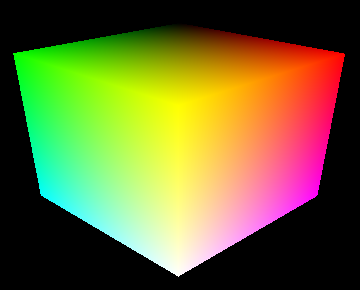
\includegraphics[scale = 0.5]{1.png}
  \caption{Resultados}
 \end{figure}

 \item \textbf{Modifique el código anterior, de tal manera que pueda visualizar y rotar una pirámide}
 
 Se utiliza la misma estructura del código anterior, añadiendo una función para dibujar las caras triangulares de la pirámide.
 
 \begin{lstlisting}
#include <GL/glut.h>

GLfloat color[5][3] =
{
	{1.0,0.0,0.0},
	{1.0,1.0,0.0},
	{0.0,1.0,0.0},
	{0.0,0.0,1.0},
	{1.0,0.0,1.0},
};

float ver[5][3] =
{
	{-1.0,-1.0,-1.0},
	{-1.0,1.0,-1.0},
	{1.0,1.0,-1.0},
	{1.0,-1.0,-1.0},
	{0.0,0.0,1.0},
};

void quad(int a, int b, int c, int d){
	glBegin(GL_QUADS);
		glColor3fv(color[a]);
		glVertex3fv(ver[a]);
		glColor3fv(color[b]);
		glVertex3fv(ver[b]);
		glColor3fv(color[c]);
		glVertex3fv(ver[c]);
		glColor3fv(color[d]);
		glVertex3fv(ver[d]);
	glEnd();
}

void triangle(int a, int b, int c){
	glBegin(GL_TRIANGLES);
		glColor3fv(color[a]);
		glVertex3fv(ver[a]);
		glColor3fv(color[b]);
		glVertex3fv(ver[b]);
		glColor3fv(color[c]);
		glVertex3fv(ver[c]);
	glEnd();
}

void colorPiramid(){
	quad(0,3,2,1);
	triangle(0,4,1);
	triangle(1,4,2);
	triangle(2,4,3);
	triangle(3,4,0);
}

double rotate_y = 0;
double rotate_x = 0;

void specialKeys(int key, int x, int y){
	if(key == GLUT_KEY_RIGHT) rotate_y += 5;
	else if(key == GLUT_KEY_LEFT) rotate_y -=5;
	else if(key == GLUT_KEY_UP) rotate_x +=5;
	else if(key == GLUT_KEY_DOWN) rotate_x -= 5;
	glutPostRedisplay();
}
void display(){
	glClearColor(0,0,0,1);
	glClear(GL_COLOR_BUFFER_BIT | GL_DEPTH_BUFFER_BIT);
	glMatrixMode(GL_PROJECTION);
	glLoadIdentity();
	int w = glutGet(GLUT_WINDOW_WIDTH);
	int h = glutGet(GLUT_WINDOW_HEIGHT);
	gluPerspective(60, w/h, 0.1, 100);
	glMatrixMode(GL_MODELVIEW);
	glLoadIdentity();
	gluLookAt(3,3,3,
			  0,0,0,
			  0,0,1);
	glRotatef(rotate_x, 1.0, 0.0, 0.0);
	glRotatef(rotate_y, 0.0, 1.0, 0.0);
	colorPiramid();
	glutSwapBuffers();
}

int main(int argc, char ** argv){
	glutInit(&argc, argv);
	glutInitDisplayMode(GLUT_RGBA | GLUT_DEPTH | GLUT_DOUBLE);
	glutInitWindowSize(640, 480);
	glutCreateWindow("GLUT");
	glutDisplayFunc(display);
	glutSpecialFunc(specialKeys);
	glEnable(GL_DEPTH_TEST);
	glutMainLoop();
	return 0;
}
 \end{lstlisting}

 \begin{figure}[H]
  \centering
  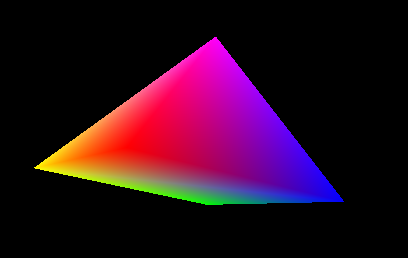
\includegraphics[scale = 0.5]{2.png}
  \caption{Resultados}
 \end{figure}
 
 \item \textbf{Modifique el código anterior, de tal manera que puede visualizar y rotar un cilindro}
 
 Se dibuja un circulo por segmentos y se refleja para dibujar el segundo circulo del cilindro. Luego se unen los dos círculos mediante rectángulos.
 
 \begin{lstlisting}
#include <GL/glut.h>
#include <iostream>
#include <cmath>
#include <vector>
#include <tuple>

using namespace std;

GLfloat color[5][3] =
{
	{1.0,0.0,0.0},
	{1.0,1.0,0.0},
	{0.0,1.0,0.0},
	{0.0,0.0,1.0},
	{1.0,0.0,1.0},
};

void drawCilindro(float cx, float cy, float r, float z,  int num_segments) 
{ 
	float theta = 2 * 3.1415926 / float(num_segments); 
	float tangetial_factor = tanf(theta);
	float radial_factor = cosf(theta);
	float x = r;
	float y = 0; 
	vector<tuple<float,float,float>> puntos;
	glColor3fv(color[1]);
	glBegin(GL_POLYGON);
		for(int i = 0; i < num_segments; i++) 
		{ 
			puntos.push_back(make_tuple(x + cx, y + cy, z));
			glVertex3f(x + cx, y + cy, z);
			float tx = -y; 
			float ty = x; 
			x += tx * tangetial_factor; 
			y += ty * tangetial_factor;  
			x *= radial_factor; 
			y *= radial_factor;
		} 
	glEnd(); 
	glBegin(GL_POLYGON);
		for(int i = 0; i < puntos.size(); i++){
			tie(x,y,z) = puntos[i];
			z += 2;
			glVertex3f(x,y,z);
		}
	glEnd();
	glColor3fv(color[2]);
	float antX, antY, antZ;
	float actualX, actualY, actualZ;
	tie(antX,antY,antZ) = puntos[0];
	for(int i = 1; i < puntos.size(); i++){
		tie(actualX, actualY, actualZ) = puntos[i];
		glBegin(GL_QUADS);
			glVertex3f(antX,antY,antZ);
			glVertex3f(antX,antY,antZ + 2);
			glVertex3f(actualX, actualY, actualZ + 2);
			glVertex3f(actualX, actualY, actualZ);
		glEnd();
		antX = actualX;
		antY = actualY;
		antZ = actualZ;
	}
	tie(actualX, actualY, actualZ) = puntos[0];
	glBegin(GL_QUADS);
		glVertex3f(antX,antY,antZ);
		glVertex3f(antX,antY,antZ + 2);
		glVertex3f(actualX, actualY, actualZ + 2);
		glVertex3f(actualX, actualY, actualZ);
	glEnd();
}

double rotate_y = 0;
double rotate_x = 0;

void specialKeys(int key, int x, int y){
	if(key == GLUT_KEY_RIGHT) rotate_y += 5;
	else if(key == GLUT_KEY_LEFT) rotate_y -=5;
	else if(key == GLUT_KEY_UP) rotate_x +=5;
	else if(key == GLUT_KEY_DOWN) rotate_x -= 5;
	glutPostRedisplay();
}
void display(){
	glClearColor(0,0,0,1);
	glClear(GL_COLOR_BUFFER_BIT | GL_DEPTH_BUFFER_BIT);
	glMatrixMode(GL_PROJECTION);
	glLoadIdentity();
	int w = glutGet(GLUT_WINDOW_WIDTH);
	int h = glutGet(GLUT_WINDOW_HEIGHT);
	gluPerspective(60, w/h, 0.1, 100);
	glMatrixMode(GL_MODELVIEW);
	glLoadIdentity();
	gluLookAt(3,3,3,
			  0,0,0,
			  0,0,1);
	glRotatef(rotate_x, 1.0, 0.0, 0.0);
	glRotatef(rotate_y, 0.0, 1.0, 0.0);
	drawCilindro(0,0,1,-1.0, 100);
	glutSwapBuffers();
}

int main(int argc, char ** argv){
	glutInit(&argc, argv);
	glutInitDisplayMode(GLUT_RGBA | GLUT_DEPTH | GLUT_DOUBLE);
	glutInitWindowSize(640, 480);
	glutCreateWindow("GLUT");
	glutDisplayFunc(display);
	glutSpecialFunc(specialKeys);
	glEnable(GL_DEPTH_TEST);
	glutMainLoop();
	return 0;
}
 \end{lstlisting}

 \begin{figure}[H]
  \centering
  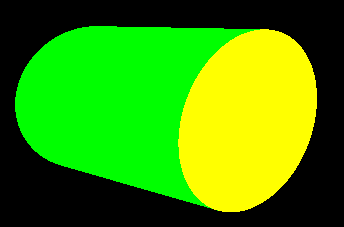
\includegraphics[scale = 0.5]{3.png}
  \caption{Resultados}
 \end{figure}

 \item \textbf{Perspectivas}
 
 \begin{itemize}
  \item \textbf{¿Qué es una proyección en perspectiva?}
  
  Es cuando un punto, polígono u objeto en el mundo real es representado en un plano de proyección en base a puntos de fuga. Dependiendo de la posición de los puntos
  de fuga y del objeto real, se tiene una proyección en el plano del objeto, que puede cambiar de tamaño y de forma.  
  \item \textbf{¿Qué es una proyección ortográfica?}
  
  Es cuando un punto, polígono u objeto en el mundo real es representado en un plano de protección en base a líneas de proyección las cuales son perpendiculares al plano.
  El tamaño no sufre cambio en tamaño ni en forma.
  \item \textbf{¿Qué aspectos se tiene que tomar en cuenta en cada caso?}
  
  En la proyección ortográfica no se necesitan muchas variables, las únicas que se necesitan son el tamaño del plano de proyección. En cambio, para la proyección en
  perspectiva si se necesitan varias variables como: el tamaño del plano de proyección, la posición del o los puntos de fuga, el ángulo de visión, la distancia del
  punto de fuga al plano y la distancia del plano al objeto real.
  \item \textbf{Escriba un código (programa) de ejemplo para cada caso}
  
  \textbf{Proyección ortográfica}
  \begin{lstlisting}
#include <GL/glut.h>
#include <iostream>

using namespace std;

GLsizei winWidth = 800, winHeight = 600;

void init(void){
    glClearColor(1.0,1.0,1.0,1.0);
    glMatrixMode(GL_PROJECTION);
    gluOrtho2D(0.0, 800.0, 0.0, 600.0);
}

void display(){
	glClear(GL_COLOR_BUFFER_BIT);
	glColor3f(1.0, 0.0, 0.0);
	glBegin(GL_QUADS);
		glVertex2i(300, 200);
		glVertex2i(300, 400);
		glVertex2i(500, 400);
		glVertex2i(500, 200);
	glEnd();
	glFlush();
}

int main(int argc, char **argv){
    glutInit(&argc, argv);
    glutInitDisplayMode(GLUT_SINGLE | GLUT_RGB);
    glutInitWindowSize(winWidth, winHeight);
    glutInitWindowPosition(100, 100);
    glutCreateWindow("GLU");
    init();
    glutDisplayFunc(display);
    glutMainLoop();
    return 0;
}
  \end{lstlisting}
  \begin{figure}[H]
   \centering
   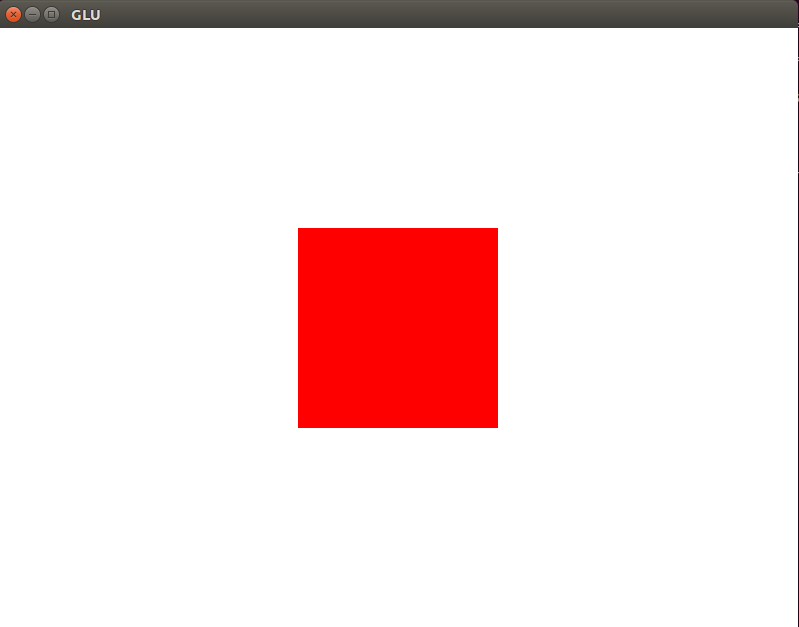
\includegraphics[scale = 0.5]{4.png}
   \caption{Proyección ortográfica}
  \end{figure}

  \textbf{Proyección en perspectiva}
  
  \begin{lstlisting}
#include <GL/glut.h>

void display(){
    glClearColor(1,1,1,1);
    glClear(GL_COLOR_BUFFER_BIT | GL_DEPTH_BUFFER_BIT);
    glMatrixMode(GL_PROJECTION);
    glLoadIdentity();
    int w = glutGet(GLUT_WINDOW_WIDTH);
    int h = glutGet(GLUT_WINDOW_HEIGHT);
    gluPerspective(60, w/h, 0.1, 100);
    glMatrixMode(GL_MODELVIEW);
    glColor3f(1.0, 0.0, 0.0);
    glLoadIdentity();
    gluLookAt(3,3,3,
              0,0,0,
              0,0,1);
    glBegin(GL_QUADS);
        glVertex2f(-1,-1);
        glVertex2f( 1,-1);
        glVertex2f( 1, 1);
        glVertex2f(-1, 1);
    glEnd();
    glutSwapBuffers();
}

int main(int argc, char ** argv){
    glutInit(&argc, argv);
    glutInitDisplayMode(GLUT_RGBA | GLUT_DEPTH | GLUT_DOUBLE);
    glutInitWindowSize(640, 480);
    glutCreateWindow("GLUT");
    glutDisplayFunc(display);
    glEnable(GL_DEPTH_TEST);
    glutMainLoop();
    return 0;
}
  \end{lstlisting}
  \begin{figure}[H]
   \centering
   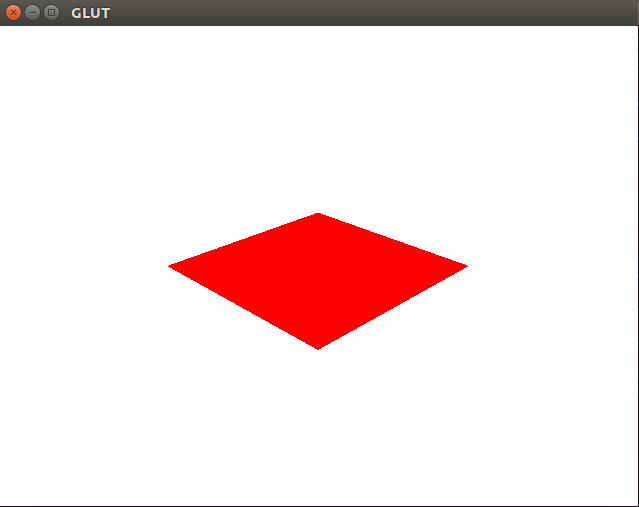
\includegraphics[scale = 0.5]{5.png}
   \caption{Proyección en perspectiva}
  \end{figure}
 \end{itemize}
\end{enumerate}


\end{document}

